\documentclass[9pt,a4paper]{extarticle}
\usepackage[margin=1.4cm]{geometry}
\usepackage{graphicx}
\usepackage{booktabs}
\usepackage{amsmath}
\usepackage[font=small,labelfont=bf,skip=2pt]{caption}
\usepackage{enumitem}
\usepackage[hidelinks]{hyperref}
\setlist{nosep,leftmargin=1.1em}
\setlength{\parindent}{0pt}
\setlength{\parskip}{2.5pt}
\usepackage{titlesec}
\titleformat{\section}{\bfseries\normalsize}{\thesection.}{0.4em}{}
\titlespacing*{\section}{0pt}{5pt}{2pt}
\pagestyle{empty}

\begin{document}
\begin{center}
{\large \textbf{IE643 Novelty Assessment Report: Trajectory-Conditioned Motion-Control Adapter for Image-to-Video Diffusion}}\\[2pt]
Team VIBE: Mithra Bijumon (24b0040), Stuti Mahajan (24b0067)
\end{center}

\section{Task and setup}
Given one image and one drawn path, generate a video in which the single object follows the path. We keep LTX-Video 2B frozen (no LoRA) and train only a small ControlNet-style adapter (5.9M parameters): a conv encoder and 2 transformer blocks on a condition (the object's SAM silhouette moved along the path, its displacement, the object's own feature), then zero-initialised projections added after every 2nd frozen block through forward hooks. The residual is multiplied by a Gaussian footprint around the object (radius $2\times$ the object) so the background gets no injection, scaled by the hidden state's RMS and capped at 5\%. Training uses a focus loss (object and background tokens averaged separately with SAM~2 masks, object weight 5). Data: 714 GOT-10k single-object clips (static camera), SAM 2 masks, Qwen2-VL-2B captions as per-clip prompts. We report object and background motion separately (CoTracker3 tracks, SAM 2 object masks).

\section{Experiments, by instructor feedback}
\textbf{Background moves with the object.} Object-only injection and the separate focus loss target this. Measuring our first injection showed a bug: the 5\% cap bounded the RMS over \emph{all} tokens, but with local injection most tokens receive zero, so tokens inside the footprint received a median $7.4\times$ the cap (3.7--16.9$\times$ per clip, 16 validation clips). This likely explains the mosaic noise of our early checkpoints. A per-token cap removes the hot spot (implemented, unit-tested). In the final recipe the cap never binds (the injection is only 0.1--0.7\% of the hidden state), so this bug did not affect the final numbers; it mattered for runs with stronger injection.\\
\textbf{Seed sensitivity.} Benchmarks use matched seeds. We found that the VAE posterior was sampled without a seed at generation time, so ``matched'' runs differed; it is now seeded (verified by a determinism test). Our final benchmark is still one seed (see limitations).\\
\textbf{Forward vs.\ backward.} Every clip is tested with left, right, up, down and diagonal paths; Table~2 reports opposite directions separately.\\
\textbf{Out-of-domain images.} The benchmark harness supports a separate clean-image group, but we have not run it yet (the benchmark below has 0 out-of-domain images).\\
\textbf{Training-free path.} We render a ``drag video'' (SAM cut-out moved along the path, hole inpainted) and start denoising from it (SDEdit, $\sigma{=}0.8$), putting back the object-free scene outside the footprint. This moves the cat and the boat cleanly; the cyclist keeps a ghost because the SAM mask (and stored box) covers only legs and bike. A faint ghost remains for the boat (Fig.~1).\\
\textbf{SDE-style training (abandoned).} We trained on samples that start from the noised drag video. Validation loss on those samples improved, but loss on normal clips got worse and generated frames were degraded at full strength or showed no benefit at reduced strength. We believe the loss gain came from learning to repaint the drag video into a real frame (averaging), not from following the path; this is a hypothesis we did not isolate. We therefore reverted to the plain recipe below.\\
\textbf{Final recipe (classic).} Footprint, displacement and object-feature condition only; global cap 0.05; lr $3{\times}10^{-5}$, batch 1, 10 epochs; focus loss on. This reconstructs our earlier run that had improved on validation; the exact code of that run was not saved, so it is rebuilt from our logs and notes.

\textbf{Other work.} \emph{Data:} GOT-10k clips filtered for camera motion, SAM masks on the first frame, SAM 2 masks on all frames, CoTracker3 tracks, per-clip captions (Qwen2-VL-2B, compared with Florence-2 on sample clips); a tool flags clips whose mask covers only part of the object (115 of 714 flagged, noisy; nothing was removed). \emph{Inference dials:} adapter strength, motion guidance, adapter active only at high noise. \emph{Metrics:} CoTracker3 (ATE, PCK, direction, progress), SAM 2 object metrics, background drift and flow, CLIP, PSNR/SSIM, warp error; 33 unit tests. The code also supports the 13B model; all reported runs use 2B because of free-compute limits.

\section{Results}
\textbf{Training validation.} On 16 held-out clips, the gain on object tokens (loss without path minus loss with path) was $-0.43{\times}10^{-3}$ at epoch 1, best $+0.01{\times}10^{-3}$ at epoch 4, worst $-1.36{\times}10^{-3}$ at epoch 6 and $-0.50{\times}10^{-3}$ at epoch 10; the background gain stayed $\approx 0$ in every epoch. The adapter adds only 0.1--0.7\% of the hidden state, so on normal validation clips it does not yet use the path reliably, and we amplify it at inference (strength dial).

\textbf{Benchmark} (classic checkpoint, strength $\times3$, 8 clips $\times$ 5 paths, 1 seed, same images, paths and seed for both rows):
\begin{center}\small
\begin{tabular}{@{}lccccccc@{}}
\toprule
Table 1 & obj\_ate$\downarrow$ & obj\_dir\_cos$\uparrow$ & obj\_progress$\uparrow$ & pck@10$\uparrow$ & bg\_drift$\downarrow$ & bg\_flow$\downarrow$ & CLIP sim\\
\midrule
Plain LTX-Video & 0.155 & 0.096 & 0.025 & 0.337 & 0.062 & 0.003 & 0.943\\
Adapter & \textbf{0.140} & \textbf{0.195} & \textbf{0.097} & \textbf{0.400} & \textbf{0.059} & 0.003 & 0.943\\
\bottomrule
\end{tabular}
\end{center}

\begin{minipage}[t]{0.5\linewidth}\vspace{0pt}
\centering\small
\begin{tabular}{@{}lcccc@{}}
\toprule
Table 2 & \multicolumn{2}{c}{obj\_dir\_cos$\uparrow$} & \multicolumn{2}{c}{obj\_ate$\downarrow$}\\
Path & plain & adapter & plain & adapter\\
\midrule
left & $-0.16$ & $-0.16$ & 0.151 & 0.150\\
right & 0.16 & \textbf{0.35} & 0.163 & \textbf{0.138}\\
up & $-0.52$ & $-0.32$ & 0.186 & 0.165\\
down & 0.52 & 0.51 & 0.133 & 0.128\\
diag & 0.48 & \textbf{0.59} & 0.143 & \textbf{0.120}\\
\bottomrule
\end{tabular}
\end{minipage}\hfill
\begin{minipage}[t]{0.47\linewidth}\vspace{0pt}
\centering
\includegraphics[width=\linewidth]{figures/Intro.png}
\captionof{figure}{Boat clip: input and path; plain LTX-Video; adapter at $\times6$ (the boat moves but is stretched); adapter with drag-video start (clean move, faint ghost).}
\end{minipage}

\begin{minipage}[t]{0.55\linewidth}\vspace{0pt}
\textbf{Reading.} The adapter follows the path better than plain LTX-Video (object error $-10\%$, direction cosine and progress roughly doubled or better, PCK@10 $+0.06$) while the background and image quality are unchanged, as designed. Plain LTX-Video's direction scores for opposite paths are exact negatives (left $-0.16$, right $+0.16$): it moves the object the same way whatever the path, so its score only reflects a fixed drift. The adapter's improvement is uneven: right and diagonal improve clearly, left does not change and up stays wrong-signed, so the forward/backward asymmetry noted by the instructor remains. Per clip the picture is mixed: large wins (clip 000504 right: ATE 0.209 $\to$ 0.037; 000542 diagonal: 0.186 $\to$ 0.062) and losses (000028 down: 0.072 $\to$ 0.129; 000128 right: 0.080 $\to$ 0.122), and in many pairs neither video moves the object (identical ATE). Figure~2 shows one such clip, the cyclist, on all five paths: the visible difference between plain LTX-Video and the adapter is small, with the rider shifted slightly towards the target on the right and diagonal paths.
\end{minipage}\hfill
\begin{minipage}[t]{0.43\linewidth}\vspace{0pt}
\centering
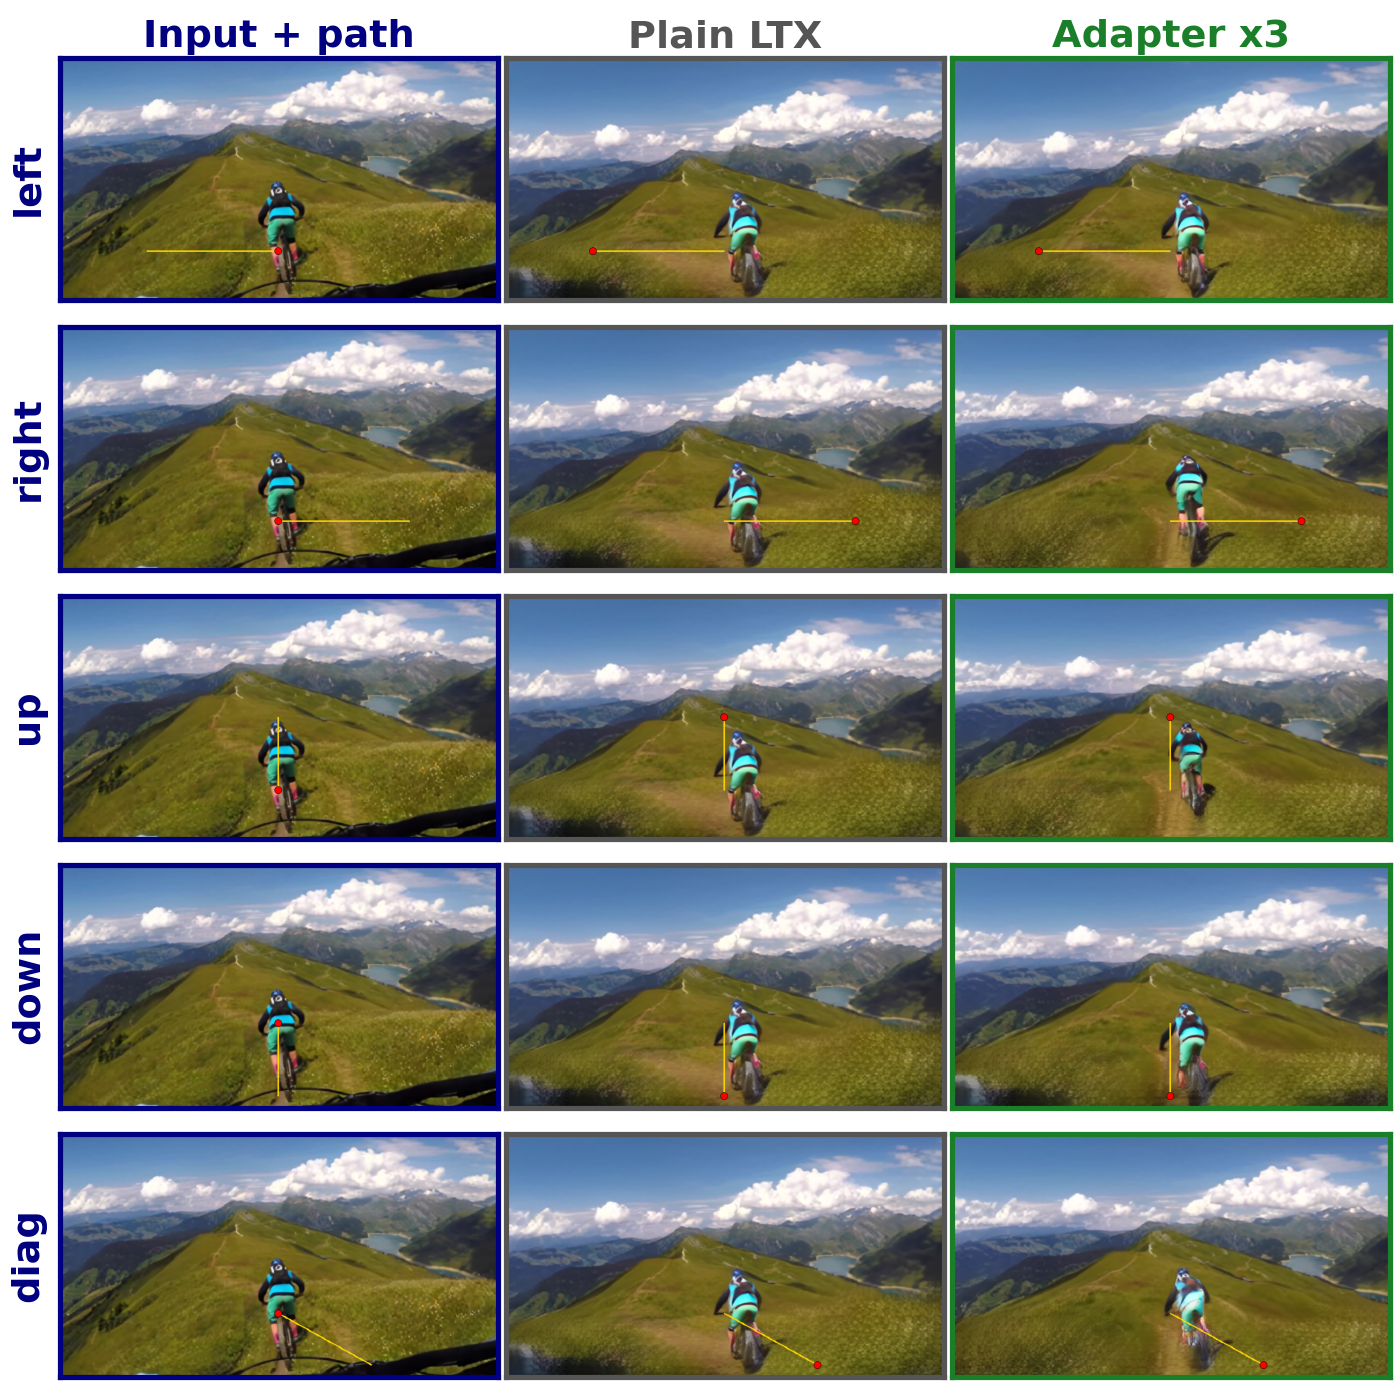
\includegraphics[width=\linewidth]{figures/Bench_cyclist.png}
\captionof{figure}{Cyclist clip, last frame, five paths (rows): input with the path, plain LTX-Video, adapter at $\times3$.}
\end{minipage}

\section{Focus loss ON vs.\ OFF}
We retrained the same recipe with the focus loss off (\texttt{--focus\_loss 0}, seed 0, 5 epochs). On the 16 validation clips (unweighted for both runs) the object-token gain was as in Table~3. The background gain is about the same in both ($+0.13$ vs.\ $+0.12\times10^{-3}$ at epoch 4). So the focus loss did not help on validation; without it the gain turned positive earlier and stayed positive.
\begin{center}\small
\begin{tabular}{@{}lccccc@{}}
\toprule
Table 3: object gain ($\times10^{-3}$) & ep.\ 1 & ep.\ 2 & ep.\ 3 & ep.\ 4 & ep.\ 5\\
\midrule
Focus ON (10-epoch schedule) & $-0.43$ & $-0.24$ & $-0.15$ & $+0.01$ & $-1.02$\\
Focus OFF (5-epoch schedule) & $-0.98$ & $-0.19$ & $+0.09$ & $+0.27$ & $+0.20$\\
\bottomrule
\end{tabular}
\end{center}
Three caveats: the differences are about $3\times10^{-4}$ from a single seed; the OFF run used a 5-epoch learning-rate schedule and the ON run a 10-epoch one, so their schedules differ; and the validation loss cannot show whether the object follows the path. Qualitatively (3 clips, right path, strengths $\times1$, $\times3$, $\times6$) the two models look alike: only the boat moves, and only at $\times6$. We have not yet benchmarked the focus-OFF model (object error, direction, background drift per path), so we make no claim about path following or the background beyond validation.

\section{Limitations and future work}
The benchmark is small (8 clips, 1 seed, no out-of-domain images) and run at a strength ($\times3$) above the trained one, so the gains are indicative, not significant. The validation gain stayed close to zero, so we do not claim the adapter learned the path robustly. Next steps: focus-loss on/off ablation, mean $\pm$ std over several seeds, out-of-domain clean images, a higher learning rate with a stronger focus loss, and fixing partial masks (the cyclist) before retraining.

\end{document}
